Jedes Minispiel ist aus drei Leveln aufgebaut, welche progressiv schwerer werden.
So dient das erste Level als Einführung in die Mechaniken des jeweiligen Minispiels.
Das zweite Level kann als \glqq standard\grqq{}-Schwierigkeitsgrad verstanden werden und im Dritten können die Spielenden dann ihre erlernten Fähigkeiten in schwierigen Herausforderungen unter Beweis stellen.
Nach dem erfolgreichen Beenden eines Levels erhält die Spielfigur ein Item, welches dann im Kampf verwendet werden kann.
Diese Items hängen von der Fachschaft und dem Schwierigkeitsgrad ab.
Die Stärke der Items skaliert also mit der Schwierigkeit des beendeten Levels. 
Da das Bearbeiten schwererer Level länger dauert, wird dies dementsprechend belohnt.\\
Im Allgemeinen soll jedes Minispiel mit einer Auswahl des Schwierigkeitsgrades beginnen, welche auch wieder verlassen werden kann, wenn sich doch gegen das Spielen entschieden wird.
Jedes Level bietet zusätzlich noch die Möglichkeit, zur Auswahl zurückzukehren.
Nach dem Abschließen des selbigen ist es ebenfalls möglich, das Level neu zu starten.


\subsection{Informatik}

Grundlegende Idee dieses Minispiels ist das \glqq Bauen\grqq{} eines Schaltkreises aus vorgegeben Logikgattern, der vorgegebene Bedingungen erfüllen soll.
Die Spielenden haben gewonnen, wenn das richtige beziehungsweise die richtigen Gatter ausgewählt wurden.
Es kann nur das erste Level verloren werden, worauf später noch eingegangen wird.\\
Die Level der Fachschaft Informatik bestehen jeweils aus zwei wesentlichen Komponenten:
Zunächst gibt es einen Schaltkreis, welcher aus Tastern, mit \glqq{}?\grqq{} verdeckten Logikgattern sowie Lämpchen aufgebaut ist.
Die zweite Komponente bilden verschiedene Logikgatter, aus welchen das im Schaltkreis verdeckte bzw. die im Schaltkreis verdeckten ausgewählt werden müssen.

\begin{figure}[H]
	\centering
	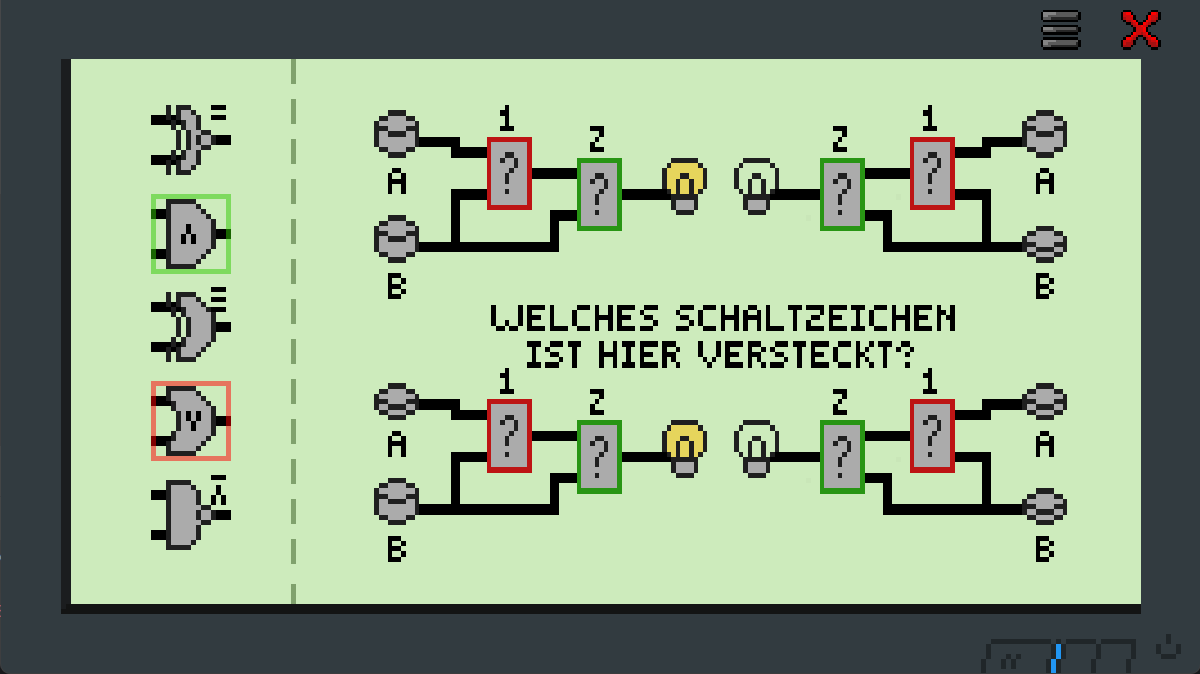
\includegraphics[width=.7\textwidth]{bilder/MinispielInformatik.png}
	\caption{Level 2 des Minispiels der Fachschaft Informatik}
	\label{fig:mginf}
\end{figure}

Verschiedene Schwierigkeiten werden auf zwei Weisen ermöglicht:

\begin{itemize}
    \item Die Anzahl an Logikgattern, aus denen ausgewählt werden kann, erhöht sich mit jedem Schwierigkeitsgrad.
            So sind es im ersten Level 4, im zweiten Level 5 und im dritten Level 6 Logikgatter, welche zur Auswahl stehen.
    \item Die Komplexität des Schaltkreises sowie die Anzahl an verdeckten Gattern ändern sich dem Schwierigkeitsgrad entsprechend.
\end{itemize}

Jedes Level verwendet außerdem, im Sinne der Variabilität, drei verschiedene Schaltkreise, aus denen bei jedem Minispiel-Start einer zufällig gewählt wird.

\subsubsection{Level 1}

Bei den Schaltkreisen des ersten Levels fehlt jeweils nur ein Logikgatter, das zwei Eingänge mit einem Ausgang verbindet.
Gesucht wird also das Logikgatter $G \in \{\land , \lor , \overline{\land}, \overline{\lor}, \veebar, \overline{\veebar}\}$\footnote{$\land = AND,\ \lor = OR,\ \overline{\land} = NAND,\ \overline{\lor} = NOR,\ \veebar = XOR,\ \overline{\veebar} = XNOR$}, welches folgende Bedingungen erfüllt:

\begin{align*}
    x_1 G x_2 = y
\end{align*}

Dadurch, dass jeder Schaltkreis zwei Eingänge und einen Ausgang besitzt, ergeben sich vier mögliche Zustände, die in Form einer Wahrheitswerttabelle dargestellt werden können.
Für die Rätsel des ersten Levels wurden folgende Tabellen festgelegt:

\begin{table}[H]
    \centering
    \begin{minipage}{.33\textwidth}
        $G = \land$\\
        \vfill
        \begin{tabular}{|c|c|c|} 
            \hline
            $x_1$ & $x_2$ & $y$ \\
            \hline\hline
            $0$ & $0$ & $0$ \\
            $0$ & $1$ & $0$ \\
            $1$ & $0$ & $0$ \\
            $1$ & $1$ & $1$ \\
            \hline
        \end{tabular}
    \end{minipage}
    \hfill
    \begin{minipage}{.32\textwidth}
        $G = \lor$\\
        \vfill
        \begin{tabular}{|c|c|c|} 
            \hline
            $x_1$ & $x_2$ & $y$ \\
            \hline\hline
            $0$ & $0$ & $0$ \\
            $0$ & $1$ & $1$ \\
            $1$ & $0$ & $1$ \\
            $1$ & $1$ & $1$ \\
            \hline
        \end{tabular}
    \end{minipage}
    \hfill
    \begin{minipage}{.33\textwidth}
        $G = \overline{\land}$\\
        \vfill
        \begin{tabular}{|c|c|c|} 
            \hline
            $x_1$ & $x_2$ & $y$ \\
            \hline\hline
            $0$ & $0$ & $1$ \\
            $0$ & $1$ & $1$ \\
            $1$ & $0$ & $1$ \\
            $1$ & $1$ & $0$ \\
            \hline
        \end{tabular}
    \end{minipage}
    \caption{Wahrheitswerttabellen für Level 1 des Informatik-Minispiels}
    \label{tab:wwt01}
\end{table}

Diese Tabellen werden den Spielenden, aufgrund der ansprechenderen Gestaltung, in Form einer Abbildung präsentiert, welche die vier Zustände des Schaltkreises darstellt.
Ebenfalls im Sinne der Gestaltung wurde auf die Konvention, die Eingänge auf der linken Seite und die Ausgänge auf der rechten Seite darzustellen, verzichtet.
In der Abbildung \ref{fig:mginf} ist dies beispielhaft anhand eines Rätsels des zweiten Levels zu erkennen.

Dieses Level kann durch das Auswählen eines falschen Gatters verloren werden, das heißt das Minispiel muss neu gestartet werden, um das Lösen durch Raten zu verhindern.
Bei den folgenden Leveln ist dies nicht der Fall, da diese schon komplex genug sind, um Raten zu verhindern.
Ein Verlieren bei Falschauswahl würde das Spielerlebnis nur verschlechtern, da dies hier eher versehentlich geschieht.
\subsubsection{Level 2}

Im zweiten Level bestehen die Schaltkreise ebenfalls aus zwei Eingängen, sowie einem Ausgang.
Der Unterschied zu Level 1 besteht hierbei darin, dass zwei Logikgatter entfernt wurden.
Durch das erste werden beide Eingänge verbunden.
Der dadurch resultierende Ausgang wird im zweiten Logikgatter wieder mit einem der Eingänge verbunden, wodurch der finale Ausgang entsteht.
Außerdem wurde zur Reduzierung der Komplexitität die Einschränkung hinzugefügt, dass sich die Gatter unterscheiden müssen.
Gesucht werden also die Logikgatter $G_1, G_2 \in \{\land , \lor , \overline{\land}, \overline{\lor}, \veebar, \overline{\veebar}\}$, welche folgende Bedingungen erfüllen:

\begin{align*}
    (x_1 G_1 x_2) G_2 x_2 &= y\\
    G_1 &\neq G_2
\end{align*}

Dadurch, dass jeder Schaltkreis auch im zweiten Level zwei Eingänge und einen Ausgang besitzt, ergeben sich wieder vier mögliche Zustände, die in Form einer Wahrheitswerttabelle dargestellt werden können.
Für die Rätsel des zweiten Levels wurden folgende Tabellen festgelegt:

\begin{table}[h!]
    \centering
    \begin{minipage}{.33\textwidth}
        $G_1 = \land$\\
        $G_2 = \overline{\lor}$
        \vfill
        \begin{tabular}{|c|c|c|} 
            \hline
            $x_1$ & $x_2$ & $y$ \\
            \hline\hline
            $0$ & $0$ & $1$ \\
            $0$ & $1$ & $0$ \\
            $1$ & $0$ & $1$ \\
            $1$ & $1$ & $0$ \\
            \hline
        \end{tabular}
    \end{minipage}
    \hfill
    \begin{minipage}{.32\textwidth}
        $G_1 = \lor$\\
        $G_2 = \veebar$
        \vfill
        \begin{tabular}{|c|c|c|} 
            \hline
            $x_1$ & $x_2$ & $y$ \\
            \hline\hline
            $0$ & $0$ & $0$ \\
            $0$ & $1$ & $0$ \\
            $1$ & $0$ & $1$ \\
            $1$ & $1$ & $0$ \\
            \hline
        \end{tabular}
    \end{minipage}
    \hfill
    \begin{minipage}{.33\textwidth}
        $G_1 = \overline{\land}$\\
        $G_2 = \lor$
        \vfill
        \begin{tabular}{|c|c|c|} 
            \hline
            $x_1$ & $x_2$ & $y$ \\
            \hline\hline
            $0$ & $0$ & $1$ \\
            $0$ & $1$ & $1$ \\
            $1$ & $0$ & $1$ \\
            $1$ & $1$ & $1$ \\
            \hline
        \end{tabular}
    \end{minipage}
    \caption{Wahrheitswerttabellen für Level 2 des Informatik-Minispiels}
    \label{tab:wwt02}
\end{table}

Diese Tabellen werden analog zu Level 1 als Abbildungen dargestellt.

\subsubsection{Level 3}

Im dritten Level bestehen die Schaltkreise aus drei Eingängen, einem Ausgang und drei entfernten Logikgattern.
Durch die ersten beiden werden jeweils zwei der Eingänge miteinander verbunden.
Die dadurch resultierenden Ausgänge werden im dritten Logikgatter verbunden, wodurch der finale Ausgang entsteht.
Gesucht werden also die Logikgatter $G_1, G_2, G_3 \in \{\land , \lor , \overline{\land}, \overline{\lor}, \veebar, \overline{\veebar}\}$, welche folgende Bedingungen erfüllen:

\begin{align*}
    (x_1 G_1 x_2) G_3 (x_2 G_2 x_3) &= y\\
    G_1 \neq G_2 &\neq G_3 
\end{align*}

Dadurch, dass jeder Schaltkreis aus drei Eingänge und einen Ausgang besteht, ergeben sich insgesamt acht mögliche Zustände, die in Form einer Wahrheitswerttabelle dargestellt werden können.
Für die Rätsel des dritten Levels wurden folgende Tabellen festgelegt:

\begin{table}[h!]
    \centering
    \begin{minipage}{.33\textwidth}
        $G_1 = \land$\\
        $G_2 = \veebar$\\
        $G_3 = \lor$
        \vfill
        \begin{tabular}{|c|c|c|c|} 
            \hline
            $x_1$ & $x_2$ & $x_3$ & $y$\\
            \hline\hline
            $0$ & $0$ & $0$ & $0$\\
            $0$ & $0$ & $1$ & $1$\\
            $0$ & $1$ & $0$ & $1$\\
            $0$ & $1$ & $1$ & $0$\\
            $1$ & $0$ & $0$ & $0$\\
            $1$ & $0$ & $1$ & $1$\\
            $1$ & $1$ & $0$ & $1$\\
            $1$ & $1$ & $1$ & $1$\\
            \hline
        \end{tabular}
    \end{minipage}
    \hfill
    \begin{minipage}{.32\textwidth}
        $G_1 = \overline{\veebar}$\\
        $G_2 = \land$\\
        $G_3 = \lor$
        \vfill
        \begin{tabular}{|c|c|c|c|} 
            \hline
            $x_1$ & $x_2$ & $x_3$ & $y$\\
            \hline\hline
            $0$ & $0$ & $0$ & $1$\\
            $0$ & $0$ & $1$ & $1$\\
            $0$ & $1$ & $0$ & $0$\\
            $0$ & $1$ & $1$ & $1$\\
            $1$ & $0$ & $0$ & $0$\\
            $1$ & $0$ & $1$ & $0$\\
            $1$ & $1$ & $0$ & $1$\\
            $1$ & $1$ & $1$ & $1$\\
            \hline
        \end{tabular}
    \end{minipage}
    \hfill
    \begin{minipage}{.33\textwidth}
        $G_1 = \veebar$\\
        $G_2 = \lor$\\
        $G_3 = \land$
        \vfill
        \begin{tabular}{|c|c|c|c|} 
            \hline
            $x_1$ & $x_2$ & $x_3$ & $y$\\
            \hline\hline
            $0$ & $0$ & $0$ & $0$\\
            $0$ & $0$ & $1$ & $0$\\
            $0$ & $1$ & $0$ & $1$\\
            $0$ & $1$ & $1$ & $1$\\
            $1$ & $0$ & $0$ & $0$\\
            $1$ & $0$ & $1$ & $1$\\
            $1$ & $1$ & $0$ & $0$\\
            $1$ & $1$ & $1$ & $0$\\
            \hline
        \end{tabular}
    \end{minipage}
    \caption{Wahrheitswerttabellen für Level 3 des Informatik-Minispiels}
    \label{tab:wwt03}
\end{table}

Da die Wahrheitswerttabellen des dritten Levels acht Zustände beinhalten, wird auf die Darstellung jedes einzelnen Zustandes verzichtet und nur der erste Zustand als Schaltkreis abgebildet.
Die anderen werden als Tabelle präsentiert.

\subsubsection{Reflexion}

Bei dem Minispiel der Fachschaft Informatik wird die Theorie spielerisch mit der Praxis verbunden.
Die Spielenden werden mit abstrakten boolschen Operationen sowie mit erwarteten Ergebnissen konfrontiert und können ihre Überlegungen dann anhand von Logikgattern und Schaltkreisen in die Tat umsetzten.
Es fördert vor allem logisches Denken, jedoch auch die Fähigkeit, mit begrenzten Mitteln ein gewünschtes Ergebnis zu erziehlen.
Außerdem regen die Rätsel durch ihre Komplexitität dazu an, Lösungsstrategien zu entwickeln, anstatt Antwortmöglichkeiten einfach auszuprobieren oder gar zu raten.\\
Das erste Level bietet einen guten Einstieg in die Funktionsweise des Spieles, da hier nur die Eigenschaften der einzelnen Gatter abgefragt und diese noch nicht verkettet werden.
Der Schwierigkeitsgrad nimmt im zweiten Level deutlich zu, jedoch kann hier durch Überlegungen, die zur Vereinfachungen des Problemes führen\footnote{Beispielsweise folgende Aussage: \glqq Der Ausgang ist in jedem Fall gleich Eingang 1.\grqq} dennoch gut eine Lösung gefunden werden.
Das dritte Level ist sehr komplex.
Es verlangt das Verbinden dreier Gatter miteinander, was definitiv über den Rahmen eines schnellen Minispiels hinausreicht.
Hier kann zwar analog zu Level 2 vereinfacht werden, jedoch bleibt das Problem dadurch dennoch sehr schwierig.
Eine Mögliche Lösung wäre das Vorgeben eines oder mehrerer Gatter, ähnlich zum in \ref{sec:mathematics} beschriebenen Mathe-Minispiel.
Auch denkbar wäre eine Einschränkung der Antwortmöglichkeiten.
So könnten die richtigen Gatter schon gegeben sein, müssten jedoch noch an die richtige Stelle plaziert werden.\\
Das Minispiel birgt neben der Schwierigkeit auch anderweitig Potential zur Verbesserung.
Die Grafiken der Logikgatter sind schwer zuzuordnen und setzten die Kenntnis ihrer Funktionsweise vorraus.
Dies könnte mit kleinen Erklärtexten oder Beispielabbildungen behoben werden.
Zusätzlich ist das wiederholte Spielen nur begrenzt möglich.
Zwar bieten die verschiedenen Schaltkreise Variabilität, jedoch ist diese aufgrund der Menge an Rätseln sehr eingeschränkt.
Die insgesamt neun Schaltkreise können schnell auswendig gelernt werden, wodurch das Spiel seine Tiefe verliert.
Dies könnte möglicherweise mit zufällig generierten Wahrheitswerttabellen behoben werden.
Jedoch ist dabei zu beachten, dass viele Tabellen keine oder mehrere Lösungen für den gegebenen Aufbau besitzen.
Es würde sich eher anbieten das Grundkonzept zu überarbeiten, da dieses generell wenig Variabilität bietet.

\subsection{Mathematik}
\label{sec:mathematics}

Die grundlegende Idee dieses Minispiels basiert auf dem chinesischen Legespiel \glqq Tangram\grqq\footnote{Seite „Tangram“. In: Wikipedia - Die freie Enzyklopädie. Bearbeitungsstand: 17. Januar 2025, 11:35 UTC. URL: https://de.wikipedia.org/w/index.php?title=Tangram\&oldid=252340816 (Abgerufen: 14. April 2026, 11:30 UTC)}.
Hierbei wird versucht aus gegebenen Steinen eine gegeben Form zu legen.
Die Spielenden haben gewonnen, wenn die Form zu 95\% mit Steinen bedeckt ist, um das Spielerlebnis angenehmer zu gestalten, da die Steine so nicht exakt am richtigen Platz liegen müssen.
Diese Überprüfung soll automatisch beim Platzieren der Steine ablaufen, um so das Drücken eines \glqqÜberprüfungs\grqq{}-Knopfes zu ersparen.
Das Minispiel kann nicht verloren werden.\\
Die Level der Fachschaft Mathematik bestehen ebenfalls aus zwei wesentlichen Komponenten:
Zunächst gibt es einen Satz an Tangram-Steinen, welche durch Verschieben und Rotieren in eine vorgegebene Silhouette, welche die zweite Komponente darstellt, gelegt werden müssen.
Außerdem werden zufällig gewählte Steine bereits an die richtige Position platziert, um das Lösen zu vereinfachen.

\begin{figure}[H]
	\centering
	\includegraphics[width=.7\textwidth]{bilder/MinispielMathematik.png}
	\caption{Level 2 des Minispiels der Fachschaft Mathematik}
	\label{fig:mgma}
\end{figure}


Verschiedene Schwierigkeiten werden auf zwei Weisen ermöglicht:

\begin{itemize}
    \item Die Anzahl an bereits richtig angeordneten Tangram-Steinen, verringert sich mit jedem Schwierigkeitsgrad.
            So sind es im ersten Level zwei vorgegebene Steine, im zweiten Level ein und im dritten Level kein vorgegebener Stein.
    \item Die Komplexitität der Silhouette ändert sich dem Schwierigkeitsgrad entsprechend.
\end{itemize}

Jedes Level verwendet außerdem, im Sinne der Variabilität, drei verschiedene Silhouetten, aus denen bei jedem Minispiel-Start eine zufällig gewählt wird.

\subsubsection{Level 1}

Im folgenden sind die Puzzle des ersten Levels mit einer beispielhaften Lösung abgebildet.

\begin{figure}[H]
    \centering
    \begin{minipage}{0.33\textwidth}
        
\includegraphics[width=1\textwidth]{bilder/TangramHerz.png}
        \caption{Herz}
        \label{fig:therz}
    \end{minipage}
    \hfill
    \begin{minipage}{0.32\textwidth}
        
\includegraphics[width=1\textwidth]{bilder/TangramSchwan.png}
        \caption{Schwan}
        \label{fig:tschwan}
    \end{minipage}
    \hfill
    \begin{minipage}{0.33\textwidth}
        
\includegraphics[width=1\textwidth]{bilder/TangramBerg.png}
        \caption{Berg}
        \label{fig:tberg}
    \end{minipage}
\end{figure}

\subsubsection{Level 2}

Im folgenden sind die Puzzle des zweiten Levels mit einer beispielhaften Lösung abgebildet.

\begin{figure}[H]
    \centering
    \begin{minipage}{0.33\textwidth}
        
\includegraphics[width=1\textwidth]{bilder/TangramHaus.png}
        \caption{Haus}
        \label{fig:thaus}
    \end{minipage}
    \hfill
    \begin{minipage}{0.32\textwidth}
        
\includegraphics[width=1\textwidth]{bilder/TangramNinjastern.png}
        \caption{Ninjastern}
        \label{fig:tninjastern}
    \end{minipage}
    \hfill
    \begin{minipage}{0.33\textwidth}
        
\includegraphics[width=1\textwidth]{bilder/TangramBaum.png}
        \caption{Baum}
        \label{fig:tbaum}
    \end{minipage}
\end{figure}

\subsubsection{Level 3}

Im folgenden sind die Puzzle des dritten Levels mit einer beispielhaften Lösung abgebildet.

\begin{figure}[H]
    \centering
    \begin{minipage}{0.33\textwidth}
        
\includegraphics[width=1\textwidth]{bilder/TangramLäufer.png}
        \caption{Läufer}
        \label{fig:tlaeufer}
    \end{minipage}
    \hfill
    \begin{minipage}{0.32\textwidth}
        
\includegraphics[width=1\textwidth]{bilder/TangramKamel.png}
        \caption{Kamel}
        \label{fig:tkamel}
    \end{minipage}
    \hfill
    \begin{minipage}{0.33\textwidth}
        
\includegraphics[width=1\textwidth]{bilder/TangramHai.png}
        \caption{Hai}
        \label{fig:thai}
    \end{minipage}
\end{figure}

\subsubsection{Reflexion}

Das Minispiel der Fachschaft Mathematik nutz das seit Jahrhunderten bewährte chinesische Legespiel \glqq Tangram\grqq{} um das räumliche Denken der Spielenden auf die Probe zu stellen.
Es mag sehr simple erscheinen, besitzt jedoch viele mathematische Rafinessen, welche teilweise auch in unserem Schulhaus beleuchtet werden. 
Es fördert neben dem bereits Genannten ebenfalls die Fähigkeit Strukturen zu erkennen und diese zu verallgemeinern.
Die meißten Tangramsteine können als eine Kombination anderer dargestellt werden, wodurch sowohl Vielfalt, als auch Restriktion entsteht.
Sollte beispielsweise ein großer Stein übrig sein, jedoch nur kleine freie Plätze, kann versucht werden bereits platzierte Steine durch den Übrigen zu ersetzten und mit den frei gewordenen Steinen die Lücken zu füllen.\\
Die einzelnen Level unterscheiden sich wenig voneinander.
Die Schwierigkeit des Lösens eines einzelnen Puzzles ist sehr subjektiv und lässt sich so schwer festlegen, weswegen die Zuteilung der Puzzle zu den jeweilligen Level nicht sinnvoll ist.
Besser wäre es diese Levelübergreifend zu definieren und so die Schwierigkeit nur durch die Anzahl der vorgegebenen Steine zu differenzieren.
Jedoch wirft auch dies Probleme auf:
Die Schwierigkeitsänderung zwischen den Leveln ist eher gering.
So kann es beispielsweise vorkommen, dass der im zweiten Level bereits platzierte Stein so gegeben ist, dass die Platzierung eines zweiten offensichtlich erscheint\footnote{Beispielsweise das Quadrat in Abbildung \ref{fig:tninjastern}, welches die Platzierung des orangenen Dreiecks vorgeben würde.}, wodurch das Lösen des Puzzles nicht schwerer, als im ersten Level ist.
Außerdem ist diese Art des Erschwerens nicht beliebig skalierbar, da nicht weniger als kein Stein vorgegeben werden kann.\\
Das dritte Level entspricht nicht vollständig dem Bild einer schwierigen Herausforderung, weil es sich, wie bereits genannt, wenig von den anderen Leveln unterscheidet und das Lösen auch etwas zu einfach ist.
Es müsste also erschwert werden, was durch das aktuelle System nicht gewährleistet werden kann.
Eine mögliche Lösung wäre das Einführen eines zweiten Tangram-Sets, wodurch deutlich komplexere Figuren möglich werden und so auch der Unterschied zu den vorherigen Schwierigkeitsgraden deutlich wird. 